\chapter[Proposta de solução]{Proposta de solução}

\section[Motivação]{Motivação}
A motivação para desenvolver uma aplicação descentralizada  de aprendizado online reside no fato de, no cenário atual, a maioria das soluções existentes para compartilhamento de materiais educativos dependerem de infraestruturas centralizadas, que pode expor os dados a riscos de controle excessivo, censura e até indisponibilidade de acesso.

Com isso, a proposta consiste em desenvolver uma aplicação capaz de reverter este cenário, proporcionando um ambiente onde os criadores de conteúdo têm controle total sobre seus materiais, sem o risco de ser censurado. Os usuários, por sua vez, podem acessar informações de maneira segura, resiliente e de qualquer lugar do mundo.

\section[Arquitetura do sistema]{Arquitetura do sistema}

A arquitetura proposta segue o modelo Cliente-Servidor, mostrando-se ideal para o gerenciamento de usuários, bem como pelo servidor para a geração de páginas estáticas de conteúdo, que serão armazenadas na rede IPFS.

A Figura \ref{fig:arquitetura_sistema} apresenta a arquitetura do sistema projetada para o desenvolvimento da aplicação. Essa arquitetura foi concebida para garantir escalabilidade, segurança e descentralização, alinhando-se aos requisitos definidos na proposta.

% \begin{figure}[h!]
%     \centering
%     % 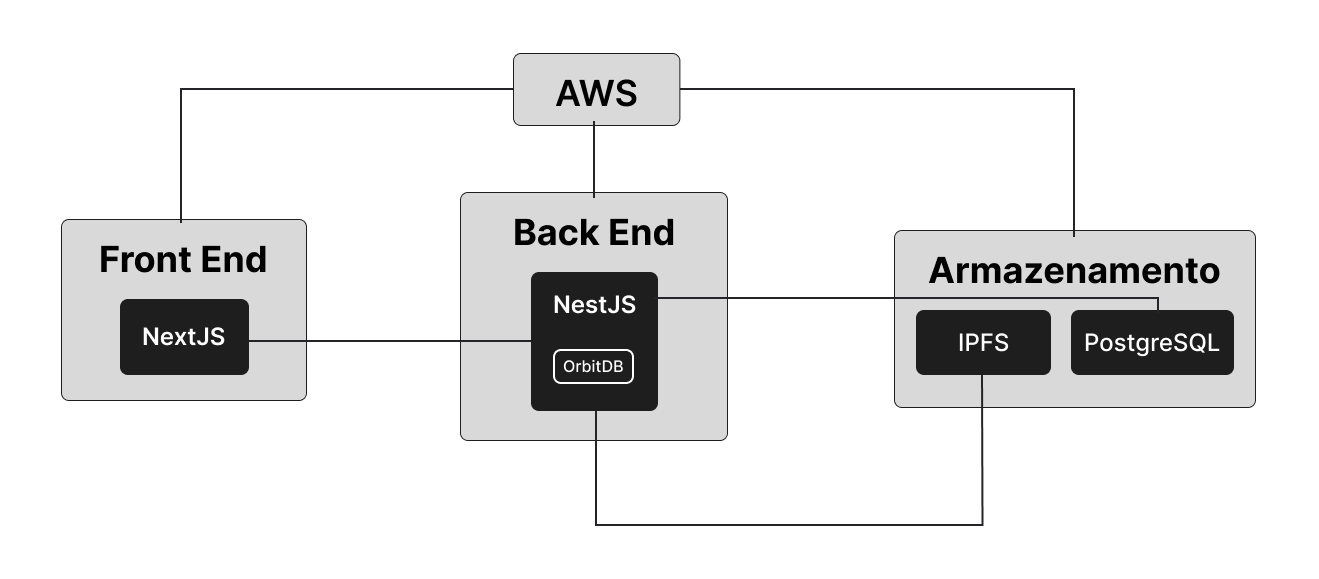
\includegraphics[width=\textwidth]{arquitetura.png}
%     \caption{Arquitetura do sistema.}
%     \label{fig:arquitetura_sistema}
% \end{figure}


